\section{DVOJRAMPOVÝ OSCILÁTOR S VCO CHARAKTERISTIKOU}
Nastaveni střídy oscilátoru, výpočet kmitočtu oscilátoru, nastavení minimální a maximální frekvence oscilátoru s ohledem na řídící napětí

\begin{figure}[h]
   \begin{center}
     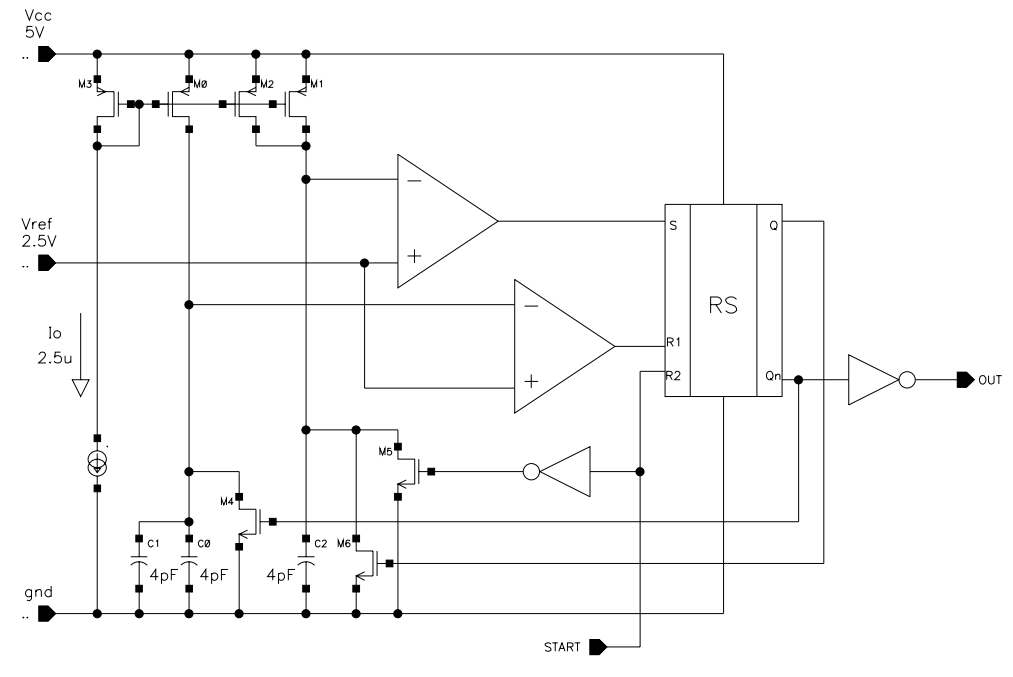
\includegraphics[scale=0.4]{images/OSC.png}
   \end{center}
   \caption{Dvourampový oscilátor}
\end{figure}

\subsection{Výpočet kmitočtu a nastavení střídy}

\begin{equation}
T_{1} = \frac{U_{ref}*C}{I}
\end{equation}
U této části periody se uplatňuje dvojice paralelních kondenzátorů, výsledná kapacita tedy bude 2*4 pF = 8 pF. Proud přes PMOS proudové zrcadlo se pouze zrcadlí jedenkrát,tedy I = 2,5 $\mu$A. 
\begin{equation*}
T_{1} = \frac{2,5*8*10^{-12}}{2,5*10^{-6}} = 8 us
\end{equation*}

Pro druhou část periody platí analogicky totéž, ovšem pro jiné hodnoty (viz. schéma).

\begin{equation*}
T_{2} = \frac{U_{ref}*C}{I} = \frac{2,5*4*10^{-12}}{5*10^{-6}} = 2 us
\end{equation*}

Kmitočet se poté vypočítá z převrácené hodnoty celé periody:

\begin{equation*}
f = \frac{1}{T_{1}+T_{2}} =  \frac{1}{8*10^{-6}+2*10^{-6}} = 100 kHz
\end{equation*}
